\documentclass[aspectratio=169,9pt]{beamer}

% ── Theme ─────────────────────────────────────────────────────────────────────
\usetheme{Madrid}
\usecolortheme{seahorse}
\usefonttheme{professionalfonts}
\setbeamertemplate{navigation symbols}{}
\setbeamertemplate{footline}[frame number]
\setbeamertemplate{itemize items}[circle]
\setbeamertemplate{enumerate items}[default]

% ── Packages ──────────────────────────────────────────────────────────────────
\usepackage[T1]{fontenc}
\usepackage[utf8]{inputenc}
\usepackage[english]{babel}
\usepackage{lmodern}
\usepackage{microtype}
\usepackage{graphicx}
\usepackage{booktabs}
\usepackage{tabularx}
\usepackage{multirow}
\usepackage{amsmath,amssymb}
\usepackage{xcolor}
\usepackage{listings}
\usepackage{tikz}
\usepackage{pgfplots}
\usepackage{fontawesome5}
\usepackage{tcolorbox}
\pgfplotsset{compat=1.18}
\usetikzlibrary{shapes.geometric, arrows.meta, positioning, fit, backgrounds, decorations.pathreplacing}

% ── Colour palette ────────────────────────────────────────────────────────────
\definecolor{primary}{RGB}{31,73,125}
\definecolor{accent}{RGB}{0,144,188}
\definecolor{success}{RGB}{40,167,69}
\definecolor{warning}{RGB}{255,153,0}
\definecolor{danger}{RGB}{220,53,69}
\definecolor{light}{RGB}{248,249,250}
\definecolor{mygray}{RGB}{108,117,125}

\setbeamercolor{palette primary}{bg=primary,fg=white}
\setbeamercolor{palette secondary}{bg=accent,fg=white}
\setbeamercolor{palette tertiary}{bg=primary!80,fg=white}
\setbeamercolor{title}{fg=white}
\setbeamercolor{frametitle}{bg=primary,fg=white}
\setbeamercolor{block title}{bg=accent,fg=white}
\setbeamercolor{block body}{bg=accent!8,fg=black}
\setbeamercolor{block title alerted}{bg=danger,fg=white}
\setbeamercolor{block body alerted}{bg=danger!8,fg=black}
\setbeamercolor{block title example}{bg=success,fg=white}
\setbeamercolor{block body example}{bg=success!8,fg=black}

% ── tcolorbox styles ──────────────────────────────────────────────────────────
\tcbuselibrary{skins,breakable}
\newtcolorbox{keybox}[1][]{
  colback=accent!10, colframe=accent, fonttitle=\bfseries\small,
  boxrule=0.8pt, arc=4pt, #1
}
\newtcolorbox{resultbox}[1][]{
  colback=success!8, colframe=success, fonttitle=\bfseries\small,
  boxrule=0.8pt, arc=4pt, #1
}

% ── Code style ────────────────────────────────────────────────────────────────
\lstset{
  basicstyle=\ttfamily\tiny,
  breaklines=true,
  backgroundcolor=\color{light},
  keywordstyle=\color{primary}\bfseries,
  commentstyle=\color{mygray},
  stringstyle=\color{warning!80!black},
  frame=tb, rulecolor=\color{accent!50},
  numbers=left, numberstyle=\tiny\color{mygray},
}

% ─────────────────────────────────────────────────────────────────────────────
\title[PathOptLearn]{\textbf{PathOptLearn}}
\subtitle{An AI-Powered Adaptive Learning Path Optimisation System}
\author{Abderrahmane Moujar}
\institute{Department of Computer Science}
\date{\today}

% ─────────────────────────────────────────────────────────────────────────────
\begin{document}

% ══════════════════════════════════════════════════════════════════════════════
%  TITLE
% ══════════════════════════════════════════════════════════════════════════════
\begin{frame}[plain]
\titlepage
\end{frame}

% ══════════════════════════════════════════════════════════════════════════════
%  OUTLINE
% ══════════════════════════════════════════════════════════════════════════════
\begin{frame}{Outline}
\tableofcontents
\end{frame}

% ══════════════════════════════════════════════════════════════════════════════
\section{Motivation \& Problem Statement}
% ══════════════════════════════════════════════════════════════════════════════

\begin{frame}{The Online Learning Paradox}
\begin{columns}[T]
  \column{0.48\textwidth}
  \begin{alertblock}{The Problem}
    \begin{itemize}
      \item Searching \textit{``I want to learn ML''} on ChatGPT returns\\
        \textbf{90+ hours} of undifferentiated content
      \item No awareness of what the student \emph{already knows}
      \item No progression logic — no mastery gating
      \item No persistence between sessions
    \end{itemize}
  \end{alertblock}

  \column{0.48\textwidth}
  \begin{block}{Existing Solutions Fall Short}
    \begin{description}
      \item[\faGraduationCap\ MOOCs] Fixed curriculum, ignores prior knowledge
      \item[\faRobot\ LLMs] Generative but stateless, untracked
      \item[\faBook\ Search] Overwhelming, unordered, unvalidated
    \end{description}
  \end{block}
\end{columns}

\vspace{0.4cm}
\begin{keybox}[title={Learning Efficiency Gap}]
\centering
\begin{tabular}{lccc}
  \toprule
  \textbf{Topic} & \textbf{ChatGPT/YouTube} & \textbf{PathOptLearn} & \textbf{Reduction} \\
  \midrule
  Machine Learning  & 90 h  & 5 h & \textbf{94.4\%} \\
  Deep Learning     & 120 h & 7 h & \textbf{94.2\%} \\
  Quantum Computing & 200 h & 8 h & \textbf{96.0\%} \\
  \bottomrule
\end{tabular}
\end{keybox}
\end{frame}

% ══════════════════════════════════════════════════════════════════════════════
\section{System Overview}
% ══════════════════════════════════════════════════════════════════════════════

\begin{frame}{PathOptLearn at a Glance}
\begin{columns}[T]
  \column{0.52\textwidth}
  \textbf{What PathOptLearn does:}
  \begin{enumerate}
    \item \textcolor{primary}{\textbf{Diagnoses}} the student's knowledge level
    \item \textcolor{accent}{\textbf{Builds}} a targeted, gap-aware roadmap
    \item \textcolor{success}{\textbf{Delivers}} adaptive lessons from multiple sources
    \item \textcolor{warning}{\textbf{Verifies}} mastery per module ($\geq 70\%$ quiz)
    \item \textcolor{danger}{\textbf{Closes}} identified gaps with ranked resources
  \end{enumerate}

  \vspace{0.3cm}
  \textbf{Core principles:}
  \begin{itemize}
    \item \faLock\ Fully local — no cloud, no data leakage
    \item \faRecycle\ Closed-loop adaptive pipeline
    \item \faDatabase\ Persistent student state across sessions
    \item \faSearch\ Multi-source knowledge enrichment
  \end{itemize}

  \column{0.44\textwidth}
  \begin{resultbox}[title={Tech Stack at a Glance}]
    \small
    \begin{tabular}{ll}
      \textbf{API}      & FastAPI (:8000)      \\
      \textbf{UI}       & Streamlit (:8501)    \\
      \textbf{LLM}      & Ollama llama3.2:1b   \\
      \textbf{Rel. DB}  & PostgreSQL (:5432)   \\
      \textbf{Graph DB} & Neo4j (:7687)        \\
      \textbf{Deploy}   & Docker Compose       \\
    \end{tabular}
  \end{resultbox}

  \vspace{0.3cm}
  \begin{alertblock}{\faTerminal\ Single command deploy}
    \texttt{\small docker compose up --build}
  \end{alertblock}
\end{columns}
\end{frame}

% ══════════════════════════════════════════════════════════════════════════════
\section{Architecture}
% ══════════════════════════════════════════════════════════════════════════════

\begin{frame}{Micro-Service Architecture}
\begin{columns}[T]
\column{0.52\textwidth}
\centering
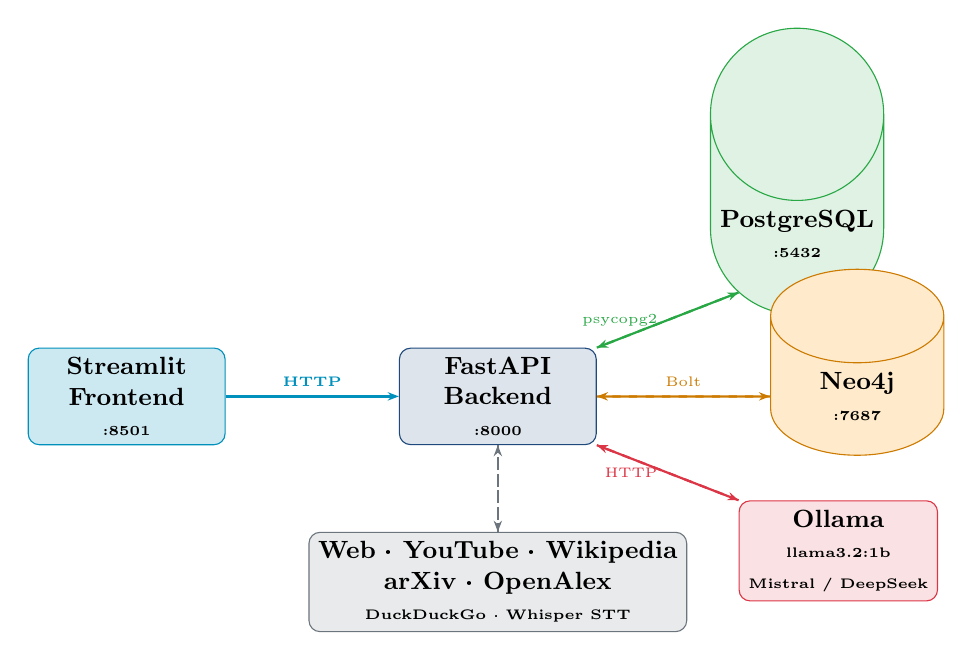
\begin{tikzpicture}[
  box/.style={rectangle, rounded corners=4pt, draw, minimum width=2.5cm,
              minimum height=0.85cm, align=center, font=\small\bfseries},
  db/.style={cylinder, draw, shape border rotate=90, minimum width=2.2cm,
             minimum height=1.0cm, align=center, font=\small\bfseries},
  arr/.style={-{Stealth[length=4pt]}, thick},
  node distance=1.2cm and 1.8cm
]
  \node[box, fill=accent!20, draw=accent]   (fe)   {Streamlit\\Frontend\\{\tiny :8501}};
  \node[box, fill=primary!15, draw=primary, right=2.2cm of fe] (api) {FastAPI\\Backend\\{\tiny :8000}};
  \node[db,  fill=success!15, draw=success, above right=0.7cm and 1.8cm of api] (pg)  {PostgreSQL\\{\tiny :5432}};
  \node[db,  fill=warning!20, draw=warning!80!black, right=2.2cm of api]        (neo) {Neo4j\\{\tiny :7687}};
  \node[box, fill=danger!15,  draw=danger,  below right=0.7cm and 1.8cm of api] (ol)  {Ollama\\{\tiny llama3.2:1b}\\{\tiny Mistral / DeepSeek}};

  \draw[arr, color=accent]           (fe)  -- node[above,font=\tiny\bfseries]{HTTP} (api);
  \draw[arr, color=success]          (api.north east) -- node[left,font=\tiny]{psycopg2} (pg.south west);
  \draw[arr, color=warning!80!black] (api) -- node[above,font=\tiny]{Bolt} (neo);
  \draw[arr, color=danger]           (api.south east) -- node[left,font=\tiny]{HTTP} (ol.north west);
  \draw[arr, dashed, color=success]  (pg.south west)  -- (api.north east);
  \draw[arr, dashed, color=warning!80!black] (neo) -- (api);
  \draw[arr, dashed, color=danger]   (ol.north west)  -- (api.south east);

  % External sources
  \node[box, fill=mygray!15, draw=mygray, below=1.1cm of api] (ext)
    {Web · YouTube · Wikipedia\\arXiv · OpenAlex\\{\tiny DuckDuckGo · Whisper STT}};
  \draw[arr, color=mygray, dashed] (api) -- (ext);
  \draw[arr, color=mygray, dashed] (ext) -- (api);
\end{tikzpicture}

\column{0.44\textwidth}
% \textbf{LLM Backend Options}

% \medskip
% \begin{tabular}{@{}ll@{}}
%   \toprule
%   \textbf{Model} & \textbf{Role} \\
%   \midrule
%   \texttt{llama3.2:1b}   & Default (fast, local) \\
%   \texttt{mistral:7b}    & Higher quality output \\
%   \texttt{deepseek-r1}   & Reasoning / advanced Q\&A \\
%   \bottomrule
% \end{tabular}

% \medskip
% \begin{keybox}[title={Whisper STT Integration}]
%   \small
%   \textbf{yt-dlp} extracts audio from YouTube\\
%   \textbf{Whisper} transcribes when no captions\\
%   $\Rightarrow$ transcript fed to LLM for quiz\\
%   \& lesson generation
% \end{keybox}

% \medskip
% \textbf{Live Knowledge Graph}\\
% {\small Neo4j — 4 topics, 35 modules,\\26 concepts, 113 edges}\\[0.2cm]
% \begin{tikzpicture}
%   \fill[danger!60]   (0,0)   circle (5pt) node[right=4pt,font=\tiny]{Topic};
%   \fill[accent!80]   (0,-0.3) circle (4pt) node[right=4pt,font=\tiny]{Module};
%   \fill[warning!80]  (0,-0.6) circle (4pt) node[right=4pt,font=\tiny]{Concept};
%   \fill[mygray!60]   (0,-0.9) circle (3pt) node[right=4pt,font=\tiny]{Resource};
% \end{tikzpicture}
\end{columns}
\end{frame}

% ── Services detail ───────────────────────────────────────────────────────────
\begin{frame}{Services in Detail}
\begin{columns}[T]
  \column{0.48\textwidth}
  \begin{block}{\faCode\ FastAPI Backend (:8000)}
    \begin{itemize}
      \item 25+ REST endpoints
      \item Full learning pipeline logic
      \item Async with Uvicorn
      \item Pydantic v2 request/response validation
      \item Auto-docs at \texttt{/docs}
    \end{itemize}
  \end{block}
  \begin{block}{\faDesktop\ Streamlit Frontend (:8501)}
    \begin{itemize}
      \item 9 learning pages + 2 utility pages
      \item Auth, Topic, Search, Quiz, Gaps,\\Roadmap, Lesson, Module Quiz, Result
      \item Knowledge Graph visualisation
      \item Progress Dashboard (4 tabs)
    \end{itemize}
  \end{block}

  \column{0.48\textwidth}
  \begin{block}{\faDatabase\ PostgreSQL (:5432)}
    \begin{itemize}
      \item 9+ tables for full learning lifecycle
      \item Per-user schemas (\texttt{user\_\{id\}}) for isolation
      \item Caches: searches, web results, lessons, reports
    \end{itemize}
  \end{block}
  \begin{block}{\faProjectDiagram\ Neo4j (:7687)}
    \begin{itemize}
      \item 5 node types, 5 relationship types
      \item Roadmap caching \& reuse
      \item Graph-aware module ordering
    \end{itemize}
  \end{block}
  \begin{block}{\faBrain\ Ollama (:11434)}
    \begin{itemize}
      \item \texttt{llama3.2:1b} local inference
      \item Quiz gen, lessons, gap analysis, ranking
    \end{itemize}
  \end{block}
\end{columns}
\end{frame}

% ── Database schemas ──────────────────────────────────────────────────────────
\begin{frame}{Database Design}
\begin{columns}[T]
  \column{0.48\textwidth}
  \textbf{PostgreSQL — 9 core tables}

  \medskip
  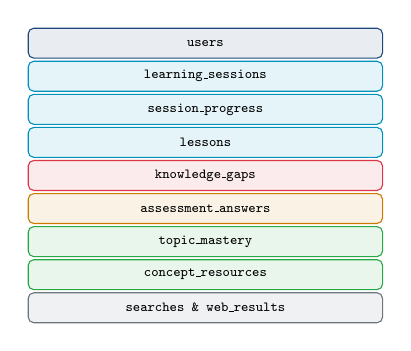
\begin{tikzpicture}[font=\tiny, node distance=0.25cm]
    \foreach \t/\c [count=\i] in {
      users/primary,
      learning\_sessions/accent,
      session\_progress/accent,
      lessons/accent,
      knowledge\_gaps/danger,
      assessment\_answers/warning!80!black,
      topic\_mastery/success,
      concept\_resources/success,
      searches \& web\_results/mygray%
    }{
      \node[rectangle, rounded corners=2pt, draw=\c, fill=\c!10,
            minimum width=4.5cm, minimum height=0.38cm,
            align=center] at (0,-\i*0.42cm) {\texttt{\t}};
    }
  \end{tikzpicture}

  \column{0.48\textwidth}
  \textbf{Neo4j — Knowledge Graph}

  \medskip
  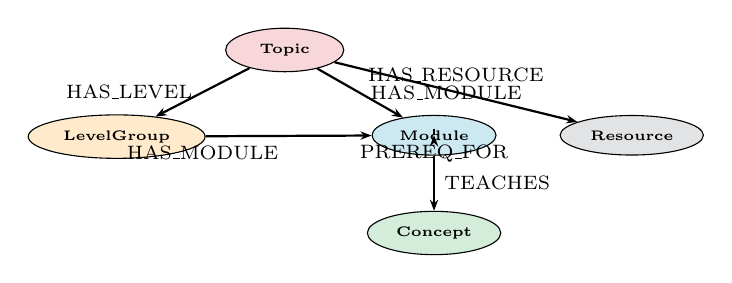
\begin{tikzpicture}[
    node/.style={ellipse, draw, fill=accent!15, font=\tiny\bfseries,
                 minimum width=1.5cm, minimum height=0.5cm, align=center},
    rel/.style={-{Stealth[length=4pt]}, thick, font=\tiny},
    node distance=0.7cm and 0.8cm
  ]
    \node[node, fill=danger!20] (t) {Topic};
    \node[node, fill=warning!20, below left=of t]  (lg) {LevelGroup};
    \node[node, fill=accent!20,  below right=of t] (m)  {Module};
    \node[node, fill=success!20, below=of m]       (c)  {Concept};
    \node[node, fill=mygray!20,  right=of m]       (r)  {Resource};

    \draw[rel] (t) -- node[left]{\scriptsize HAS\_LEVEL} (lg);
    \draw[rel] (lg) -- node[below left]{\scriptsize HAS\_MODULE} (m);
    \draw[rel] (t) -- node[right]{\scriptsize HAS\_MODULE} (m);
    \draw[rel] (m) -- node[right]{\scriptsize TEACHES} (c);
    \draw[rel] (t) -- node[above]{\scriptsize HAS\_RESOURCE} (r);
    \draw[rel, bend right=30] (m) edge node[below]{\scriptsize PREREQ\_FOR} (m);
  \end{tikzpicture}

  \medskip
  \begin{itemize}
    \item[\tiny\textbullet] Uniqueness constraints on name/uid/url
    \item[\tiny\textbullet] Cache-first lookup: $<1$s on hit
  \end{itemize}
\end{columns}
\end{frame}

% ══════════════════════════════════════════════════════════════════════════════
\section{Adaptive Learning Pipeline}
% ══════════════════════════════════════════════════════════════════════════════

\begin{frame}{7-Stage Closed-Loop Pipeline}
\centering
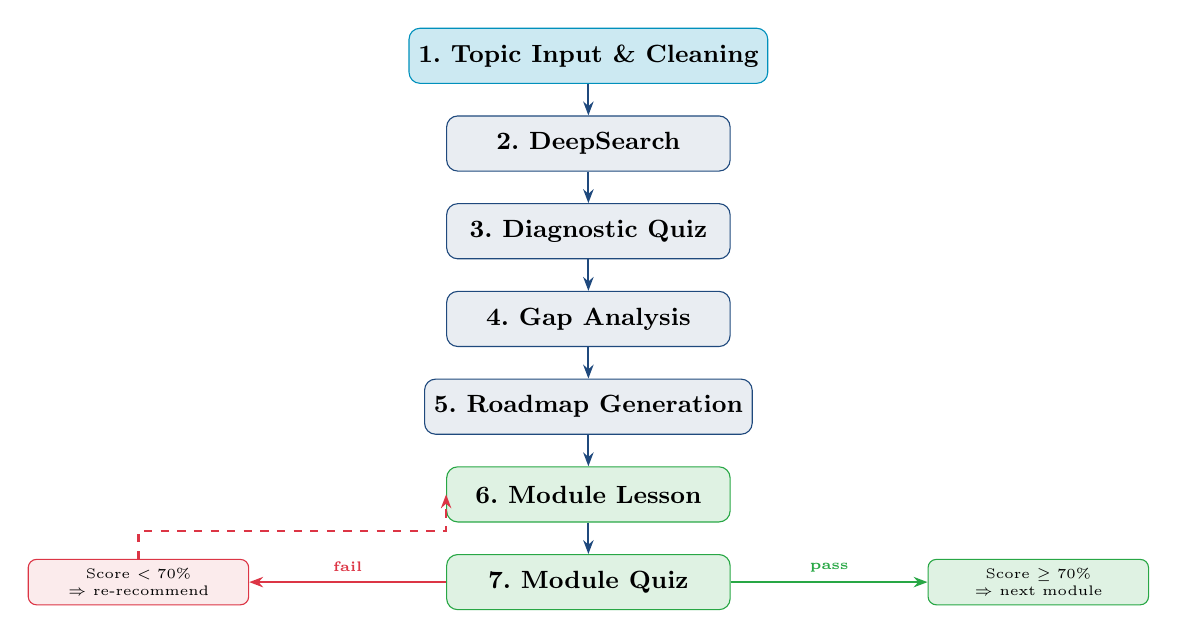
\begin{tikzpicture}[
  stage/.style={rectangle, rounded corners=4pt, draw=primary, fill=primary!10,
                minimum width=3.6cm, minimum height=0.7cm,
                font=\small\bfseries, align=center},
  arr/.style={-{Stealth[length=5pt]}, thick, color=primary},
  sub/.style={rectangle, rounded corners=3pt, draw=mygray, fill=mygray!10,
              minimum width=2.8cm, minimum height=0.5cm, font=\tiny, align=center},
  node distance=0.4cm
]
  \node[stage, fill=accent!20, draw=accent]  (s1) {1.\ Topic Input \& Cleaning};
  \node[stage, below=of s1]                  (s2) {2.\ DeepSearch};
  \node[stage, below=of s2]                  (s3) {3.\ Diagnostic Quiz};
  \node[stage, below=of s3]                  (s4) {4.\ Gap Analysis};
  \node[stage, below=of s4]                  (s5) {5.\ Roadmap Generation};
  \node[stage, fill=success!15, draw=success, below=of s5] (s6) {6.\ Module Lesson};
  \node[stage, fill=success!15, draw=success, below=of s6] (s7) {7.\ Module Quiz};

  \foreach \a/\b in {s1/s2,s2/s3,s3/s4,s4/s5,s5/s6,s6/s7}
    \draw[arr] (\a) -- (\b);

  % Pass / fail
  \node[sub, fill=success!15, draw=success, right=2.5cm of s7] (pass)
    {Score $\geq 70\%$\\ $\Rightarrow$ next module};
  \node[sub, fill=danger!10,  draw=danger, left=2.5cm of s7]  (fail)
    {Score $< 70\%$\\ $\Rightarrow$ re-recommend};
  \draw[arr, color=success] (s7.east) -- node[above, font=\tiny\bfseries]{pass} (pass.west);
  \draw[arr, color=danger]  (s7.west) -- node[above, font=\tiny\bfseries]{fail} (fail.east);
  \draw[arr, color=danger, dashed] (fail.north) -- ++(0,0.35) -| (s6.west);
\end{tikzpicture}
\end{frame}

% ── Stage 1 & 2 ───────────────────────────────────────────────────────────────
\begin{frame}{Stage 1 \& 2: Topic Input and DeepSearch}
\begin{columns}[T]
  \column{0.44\textwidth}
  \begin{block}{Stage 1 — Topic Cleaning}
    \begin{itemize}
      \item Natural-language input \\
        \small\textit{``i want to learning ML''}
      \item LLM extracts canonical name \\
        \small\textit{``Machine Learning''}
      \item Used for all subsequent Neo4j lookups
    \end{itemize}
  \end{block}

  \column{0.52\textwidth}
  \begin{block}{Stage 2 — DeepSearch (\texttt{POST /deep-search})}
    \begin{enumerate}
      \item \textbf{Cache check} — PostgreSQL hit $\Rightarrow$ instant return
      \item \textbf{Sub-queries} — LLM generates 3 targeted queries
      \item \textbf{Web search} — DuckDuckGo (6 results/query)
      \item \textbf{Open knowledge} — Wikipedia, Wikidata, OpenAlex, arXiv, DBpedia
      \item \textbf{YouTube} — \texttt{yt-dlp} + transcript (if available or whisper fallback)
      \item \textbf{Per-URL summary} — LLM summarises each source
      \item \textbf{Graph persist} — stored in PostgreSQL \& Neo4j
    \end{enumerate}
  \end{block}
\end{columns}

\vspace{0.3cm}
\begin{keybox}[title={Lesson Structure Generated by LLM}]
  \small
  Introduction $\to$ Key Concepts $\to$ Worked Examples $\to$ Common Misconceptions $\to$ Summary $\to$ Further Reading
\end{keybox}
\end{frame}

% ── Stage 3 & 4 ───────────────────────────────────────────────────────────────
\begin{frame}{Stage 3 \& 4: Diagnostic Quiz \& Gap Analysis}
\begin{columns}[T]
  \column{0.48\textwidth}
  \begin{block}{Stage 3 — Diagnostic Quiz (\texttt{GET /assess})}
    6-question MCQ with structured difficulty:
    \medskip

    \begin{tabular}{cll}
      \textcolor{success}{\faCircle} & Q1--Q2 & Basic — factual recall \\
      \textcolor{warning}{\faCircle} & Q3--Q4 & Intermediate — conceptual \\
      \textcolor{danger}{\faCircle}  & Q5--Q6 & Advanced — application \\
    \end{tabular}

    \medskip
    \begin{itemize}
      \item Each Q has a \texttt{concept} field (2--5 word label)
      \item Option \textbf{E: ``I don't know''} scores zero without penalty
    \end{itemize}

    \medskip
    \textbf{Level thresholds:}
    \begin{itemize}
      \item $0$--$40\%$ \textcolor{success}{\textbf{Beginner}}
      \item $40$--$70\%$ \textcolor{warning}{\textbf{Intermediate}}
      \item $70\%+$ \textcolor{danger}{\textbf{Advanced}}
    \end{itemize}
  \end{block}

  \column{0.48\textwidth}
  \begin{block}{Stage 4 — Gap Analysis (\texttt{POST /find-gaps})}
    \textbf{Deterministic algorithm — no LLM for scoring:}

    \begin{enumerate}
      \item Compare answers vs.\ correct answers
      \item Extract \texttt{concept} from each wrong question
      \item Assign severity:
        \begin{itemize}
          \item \texttt{advanced} $\to$ \textcolor{danger}{\textbf{High}}
          \item \texttt{intermediate} $\to$ \textcolor{warning}{\textbf{Medium}}
          \item \texttt{basic} $\to$ \textcolor{success}{\textbf{Low}}
        \end{itemize}
      \item Deduplicate \& persist to \texttt{knowledge\_gaps}
    \end{enumerate}

    \vspace{0.2cm}
    \begin{alertblock}{Design Decision}
      Scoring is \textbf{100\% deterministic} — eliminates LLM non-determinism in score reporting.
    \end{alertblock}
  \end{block}
\end{columns}
\end{frame}

% ── Stage 5 ───────────────────────────────────────────────────────────────────
\begin{frame}{Stage 5: Roadmap Generation}
\begin{columns}[T]
  \column{0.52\textwidth}
  \textbf{3-Level $\times$ 5-Module Hierarchy:}

  \medskip
  \begin{tikzpicture}[font=\small, node distance=0.35cm]
    \foreach \label/\col/\modules in {
      Beginner (M1--M5)/success/{M1,M2,M3,M4,M5},
      Intermediate (M6--M10)/warning/{M6,M7,M8,M9,M10},
      Advanced (M11--M15)/danger/{M11,M12,M13,M14,M15}
    }{
      % just show level bars
    }
    \node[rectangle, rounded corners=3pt, draw=success, fill=success!15,
          minimum width=6.5cm, minimum height=0.6cm, font=\small\bfseries]
      at (0,0) {\textcolor{success}{\faCircle} Beginner — M01--M05};
    \node[rectangle, rounded corners=3pt, draw=warning!80!black, fill=warning!15,
          minimum width=6.5cm, minimum height=0.6cm, font=\small\bfseries]
      at (0,-0.75) {\textcolor{warning!80!black}{\faCircle} Intermediate — M06--M10};
    \node[rectangle, rounded corners=3pt, draw=danger, fill=danger!15,
          minimum width=6.5cm, minimum height=0.6cm, font=\small\bfseries]
      at (0,-1.5) {\textcolor{danger}{\faCircle} Advanced — M11--M15};
    \draw[-{Stealth}, thick] (0,-0.3) -- (0,-0.45);
    \draw[-{Stealth}, thick] (0,-1.05) -- (0,-1.2);
  \end{tikzpicture}

  \medskip
  Each module contains:
  \begin{itemize}
    \item \texttt{uid}, title, objective
    \item concepts list, duration\_minutes
    \item prerequisites (for graph ordering)
  \end{itemize}

  \column{0.44\textwidth}
  \begin{block}{Generation Flow}
    \begin{enumerate}
      \item \textbf{Neo4j cache check} \\
        Returns instantly if seen before
      \item \textbf{LLM generation} \\
        Generates 5 modules per level \\ with titles, objectives, concepts
      \item \textbf{Graph persistence} \\
        Topic $\to$ LevelGroup $\to$ Module $\to$ Concept \\
        PREREQUISITE\_FOR edges added
    \end{enumerate}
  \end{block}

  \vspace{0.2cm}
  \begin{keybox}[title={Extendable to 5 levels}]
    \small Beginner $\to$ Intermediate $\to$ Advanced $\to$ Expert $\to$ Master\\
    LLM decides complexity from topic.
  \end{keybox}
\end{columns}
\end{frame}

% ── Stage 6 & 7 ───────────────────────────────────────────────────────────────
\begin{frame}{Stage 6 \& 7: Lesson, Quiz, and Mastery Loop}
\begin{columns}[T]
  \column{0.48\textwidth}
  \begin{block}{Stage 6 — Lesson (\texttt{GET /lesson})}
    \begin{enumerate}
      \item Fetch module concepts from Neo4j
      \item Run focused DeepSearch on those concepts
      \item LLM synthesises structured lesson:
        \begin{itemize}
          \item Introduction
          \item Core concepts + analogies
          \item Worked examples
          \item Misconceptions
          \item Summary + further reading
        \end{itemize}
      \item Cache in PostgreSQL \texttt{lessons} table
      \item Return lesson + resources + videos
    \end{enumerate}
  \end{block}

  \column{0.48\textwidth}
  \begin{block}{Stage 7 — Module Quiz (\texttt{POST /quiz})}
    5 MCQ questions from lesson content.

    \medskip
    \textbf{4-tier fallback generation:}
    \begin{enumerate}
      \item All 5 Qs in one LLM call
      \item One question at a time
      \item Minimal compact prompt
      \item Heuristic from key sentences
    \end{enumerate}
  \end{block}

  \begin{block}{Mastery Gate}
    \begin{center}
    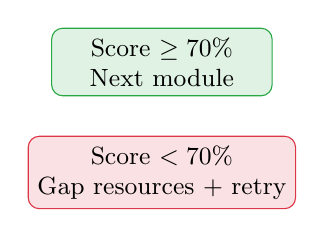
\begin{tikzpicture}[font=\small, node distance=0.5cm]
      \node[rectangle, rounded corners, draw=success, fill=success!15,
            minimum width=2.8cm, align=center]
        (pass) {Score $\geq 70\%$\\\small Next module};
      \node[rectangle, rounded corners, draw=danger, fill=danger!15,
            minimum width=2.8cm, align=center, below=of pass]
        (fail) {Score $< 70\%$\\\small Gap resources + retry};
    \end{tikzpicture}
    \end{center}
  \end{block}
\end{columns}
\end{frame}

% ── Recommender ───────────────────────────────────────────────────────────────
\begin{frame}{Resource Recommender \& Graph-Based Module Ordering}
\begin{columns}[T]
  \column{0.52\textwidth}
  \begin{block}{\texttt{GET /recommender} — Gap-Targeted Resources}
    \begin{enumerate}
      \item Look up gap concept in \texttt{concept\_resources}
      \item On cache miss: search DuckDuckGo + YouTube for\\\textit{``[concept] tutorial explained for beginners''}
      \item LLM ranks top-3 resources per gap with reason
      \item \textbf{Fallback}: return top resources if LLM rank fails
    \end{enumerate}
    \medskip
    Scoring: $p_{\text{correct}} = 1 - \text{severity\_score}$, $\;\text{severity} \in \{0.85, 0.55, 0.25, 0.10\}$
  \end{block}

  \column{0.44\textwidth}
  \begin{block}{\texttt{POST /recommend/next} — Graph + LLM Hybrid}
    \small
    \textbf{Cypher (Neo4j) scores candidates:}
    \begin{align*}
      \text{score} &= \text{concepts\_taught} \times 1.0 \\
                   &+ \text{weak\_matches} \times 2.0
    \end{align*}

    \begin{itemize}
      \item \textbf{Prerequisite guard}: skip modules with unsatisfied prerequisites
      \item \textbf{Top-10 candidates} passed to LLM
      \item LLM returns best module + personalised reason + tip
    \end{itemize}
  \end{block}
\end{columns}
\end{frame}

% ══════════════════════════════════════════════════════════════════════════════
\section{Key Features}
% ══════════════════════════════════════════════════════════════════════════════

\begin{frame}{Key Features}
\begin{columns}[T]
  \column{0.48\textwidth}

  \begin{block}{\faLock\ Fully Local \& Private}
    \begin{itemize}
      \item All LLM inference via Ollama (\texttt{llama3.2:1b})
      \item Web search via open DuckDuckGo API
      \item Zero cloud costs — \textbf{\$0 per student}
      \item Student data never leaves the machine
    \end{itemize}
  \end{block}

  \begin{block}{\faProjectDiagram\ Knowledge Graph Visualisation}
    \begin{itemize}
      \item \texttt{streamlit-agraph} interactive graph
      \item Colour-coded by node type
      \item Topic filter + node limit slider
      \item Hover shows full metadata
    \end{itemize}
  \end{block}

  \begin{block}{\faChartBar\ Progress Dashboard}
    4-tab analytics per student:
    \begin{itemize}
      \item Assessments, Gaps, Mastery, Modules
    \end{itemize}
  \end{block}

  \column{0.48\textwidth}

  \begin{block}{\faSearch\ Multi-Source Enrichment}
    \begin{itemize}
      \item DuckDuckGo (6 results/query)
      \item Wikipedia \& Wikidata (definitions)
      \item OpenAlex (open-access papers)
      \item arXiv (preprints)
      \item YouTube (tutorials + transcripts)
    \end{itemize}
  \end{block}

  \begin{block}{\faCheckCircle\ Deterministic Scoring}
    \begin{itemize}
      \item LLM \textbf{never} used for score computation
      \item Same answers always produce same level \& gaps
      \item Eliminates LLM non-determinism from assessment
    \end{itemize}
  \end{block}

  \begin{block}{\faUsers\ Per-User Schema Isolation}
    \begin{itemize}
      \item PostgreSQL schema per user (\texttt{user\_\{id\}})
      \item True multi-tenancy
      \item Private lesson history \& progress caches
    \end{itemize}
  \end{block}
\end{columns}
\end{frame}

% ══════════════════════════════════════════════════════════════════════════════
\section{System Evolution: search\_wiseper \texorpdfstring{$\to$}{->} PathOptLearn}
% ══════════════════════════════════════════════════════════════════════════════

% ── v1 overview ───────────────────────────────────────────────────────────────
\begin{frame}{search\_wiseper — v1 Prototype}
\begin{columns}[T]
  \column{0.50\textwidth}
  \begin{block}{What search\_wiseper does}
    \begin{enumerate}
      \item Student enters any \textbf{YouTube video URL}
      \item System extracts transcript:\\
        \textcolor{success}{captions first} $\to$ \textcolor{warning}{Whisper fallback}
      \item LLM (\textbf{Mistral} / \textbf{Groq llama-3.3-70b}) generates\\
        conceptual MCQ quiz from transcript
      \item Student submits answers — evaluated by LLM
      \item \textbf{LLM-driven next-video recommendation}:\\
        topic lock $\to$ query build $\to$ YouTube search\\
        $\to$ Groq picks best candidate
    \end{enumerate}
  \end{block}

  \begin{keybox}[title={3-page Streamlit App}]
    \small
    \textbf{Login} $\to$ \textbf{Dashboard} (courses \& stats) $\to$ \textbf{Learning} (video loop)
  \end{keybox}

  \column{0.46\textwidth}
  \begin{block}{Tech Stack — v1}
    \small
    \begin{tabular}{ll}
      \textbf{DB}       & SQLite (\texttt{adaptive.db}) \\
      \textbf{Auth}     & bcrypt + 6-digit code \\
      \textbf{LLM}      & Groq cloud (llama-3.3-70b) \\
                        & or fine-tuned Mistral (Colab) \\
      \textbf{Transcr.} & yt-dlp captions / Whisper \\
      \textbf{Search}   & yt-dlp YouTube search \\
      \textbf{State}    & Streamlit session only \\
    \end{tabular}
  \end{block}

  \begin{block}{Recommendation Pipeline — v1}
    \small
    \begin{enumerate}
      \item \textbf{Extract topic} (Groq, 3--5 words)
      \item \textbf{Build query} (topic + weak-concept keywords)
      \item \textbf{Search YouTube} (10 candidates, yt-dlp)
      \item \textbf{Filter captions} (prefer transcribed videos)
      \item \textbf{Groq picks best} (JSON: video\_id + reason)
    \end{enumerate}
  \end{block}
\end{columns}
\end{frame}

% ── v1 vs v2 comparison ───────────────────────────────────────────────────────
\begin{frame}{Evolution: search\_wiseper $\to$ PathOptLearn}
\small
\begin{tabularx}{\textwidth}{@{}lXX@{}}
  \toprule
  \textbf{Capability} & \textbf{search\_wiseper (v1)} & \textbf{PathOptLearn (v2)} \\
  \midrule
  Content type        & YouTube videos only           & Web + Wikipedia + arXiv + YouTube \\
  Database            & SQLite (single file)          & PostgreSQL + Neo4j (knowledge graph) \\
  LLM hosting         & Groq cloud / Colab API        & Fully local (Ollama llama3.2:1b) \\
  Diagnosis           & None (reactive only)          & 6-Q diagnostic quiz + gap analysis \\
  Roadmap             & None (video-by-video)         & 3-level $\times$ 5-module structured roadmap \\
  Mastery gating      & 60\% pass threshold           & 70\% per module + retry loop \\
  State persistence   & Streamlit session only        & PostgreSQL per-user schema + Neo4j cache \\
  Recommendation      & Rule-based query + LLM pick   & Graph Cypher scoring + LLM re-ranking \\
  Knowledge graph     & None                          & Neo4j: Topic $\to$ Module $\to$ Concept \\
  Evaluation          & None                          & KT benchmark (Riiid, EdNet, ASSISTments) \\
  Privacy             & Cloud API keys required       & Fully local, zero cost \\
  \bottomrule
\end{tabularx}

\vspace{0.2cm}
\begin{resultbox}
  search\_wiseper established the core loop — \emph{watch $\to$ quiz $\to$ recommend}. PathOptLearn generalises it to any topic, adds structured knowledge graphs, persistent state, and full local inference.
\end{resultbox}
\end{frame}

% ══════════════════════════════════════════════════════════════════════════════
\section{Advanced Retrieval: Vector DB \& Deep Learning on KG}
% ══════════════════════════════════════════════════════════════════════════════

% ── Vector DB ────────────────────────────────────────────────────────────────
\begin{frame}{Vector DB Semantic Search for Resource Retrieval}
\begin{columns}[T]
  \column{0.50\textwidth}
  \begin{block}{Limitation of Keyword Matching}
    The current \texttt{concept\_resources} cache uses \textbf{exact string matching}:
    \begin{itemize}
      \item \texttt{LOWER(topic) = LOWER(input)} in PostgreSQL
      \item Misses semantically similar queries\\
        e.g. \textit{``backprop''} $\neq$ \textit{``backpropagation algorithm''}
      \item Resource ranking is LLM-call expensive
    \end{itemize}
  \end{block}

  \begin{block}{Vector DB Architecture}
    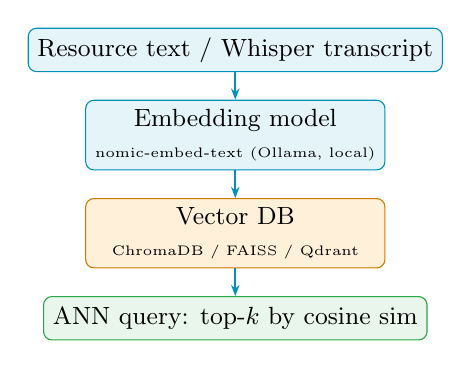
\begin{tikzpicture}[
      box/.style={rectangle, rounded corners=3pt, draw=accent, fill=accent!10,
                  minimum width=3.8cm, minimum height=0.55cm,
                  font=\small, align=center},
      arr/.style={-{Stealth[length=4pt]}, thick, color=accent},
      node distance=0.35cm
    ]
      \node[box] (r) {Resource text / Whisper transcript};
      \node[box, below=of r] (e) {Embedding model\\{\tiny nomic-embed-text (Ollama, local)}};
      \node[box, fill=warning!15, draw=warning!80!black, below=of e]
        (v) {Vector DB\\{\tiny ChromaDB / FAISS / Qdrant}};
      \node[box, fill=success!10, draw=success, below=of v]
        (q) {ANN query: top-$k$ by cosine sim};
      \draw[arr] (r)--(e); \draw[arr] (e)--(v); \draw[arr] (v)--(q);
    \end{tikzpicture}
  \end{block}

  \begin{block}{LLM Re-rank Options (all local)}
    \small
    \begin{tabular}{@{}lll@{}}
      \textbf{Model} & \textbf{Via} & \textbf{Strength} \\
      \midrule
      \texttt{llama3.2:1b} & Ollama & Fast, low RAM \\
      \texttt{mistral:7b}  & Ollama & Quality ranking \\
      \texttt{deepseek-r1} & Ollama & Reasoning chain \\
    \end{tabular}
  \end{block}

  \column{0.46\textwidth}
  \begin{block}{Integration into PathOptLearn}
    \small
    \textbf{Indexing (offline / background):}
    \begin{enumerate}
      \item \textbf{Whisper STT}: audio $\to$ transcript\\
        (fallback when no YT captions)
      \item Embed each resource summary with\\
        \texttt{nomic-embed-text} (Ollama)
      \item Store in ChromaDB / FAISS\\
        Index key: \texttt{(url, topic, type)}
    \end{enumerate}

    \medskip
    \textbf{Query (at recommendation time):}
    \begin{enumerate}
      \item Embed gap concept string
      \item ANN search: top-5 semantically similar resources
      \item Merge with Neo4j graph neighbours\\
        (concept $\to$ resource edges)
      \item Re-rank with Mistral / DeepSeek\\
        (only top-5 — 60\% fewer LLM calls)
    \end{enumerate}
  \end{block}

  \begin{resultbox}
    \small
    Whisper transcripts $+$ local embeddings $+$\\
    Mistral/DeepSeek re-rank = fully offline\\
    semantic search with no API costs.
  \end{resultbox}
\end{columns}
\end{frame}

% ── GNN on KG ────────────────────────────────────────────────────────────────
\begin{frame}{Deep Learning on the Knowledge Graph for Recommendation}
\begin{columns}[T]
  \column{0.50\textwidth}
  \begin{block}{Why Graph Neural Networks?}
    The Neo4j KG captures rich relational structure:
    \[
      \text{Topic} \xrightarrow{\text{HAS\_MODULE}} \text{Module}
      \xrightarrow{\text{TEACHES}} \text{Concept}
    \]
    Cypher scoring only uses \textbf{local hop counts} — it ignores:
    \begin{itemize}
      \item Long-range concept co-occurrence patterns
      \item Implicit difficulty ordering from student trajectories
      \item Cross-topic concept transfer (e.g. \textit{``gradient descent''} appears in ML, DL, Opt.)
    \end{itemize}
  \end{block}

  \begin{block}{Node Embedding via GNN}
    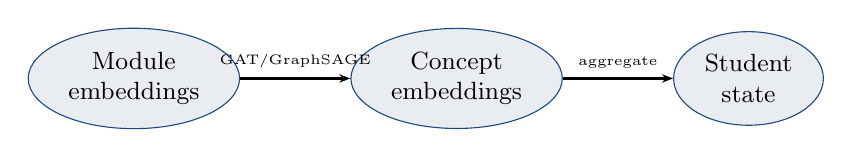
\begin{tikzpicture}[font=\small,
      n/.style={ellipse, draw=primary, fill=primary!10,
                minimum width=1.3cm, minimum height=0.45cm, align=center},
      arr/.style={-{Stealth[length=4pt]}, thick}
    ]
      \node[n] (m) {Module\\embeddings};
      \node[n, right=1.4cm of m] (c) {Concept\\embeddings};
      \node[n, right=1.4cm of c] (s) {Student\\state};
      \draw[arr] (m) -- node[above,font=\tiny]{GAT/GraphSAGE} (c);
      \draw[arr] (c) -- node[above,font=\tiny]{aggregate} (s);
    \end{tikzpicture}

    \medskip
    \small
    Each node gets a $d$-dim embedding via message passing.\\
    Student state = mean-pool of completed module embeddings.
  \end{block}

  \column{0.46\textwidth}
  \begin{block}{Training \& Recommendation}
    \small
    \textbf{Training signal:} BPR loss on (student, passed module, failed/skipped module) triples from \texttt{session\_progress}

    \[
      \mathcal{L} = -\sum_{(u,i,j)} \log \sigma\!\left(
        \mathbf{h}_u \cdot \mathbf{h}_i - \mathbf{h}_u \cdot \mathbf{h}_j
      \right)
    \]

    \medskip
    \textbf{Inference:}
    \begin{enumerate}
      \item Encode student history with GNN
      \item Score all unvisited modules:
        $\hat{r}_{ui} = \mathbf{h}_u^\top \mathbf{h}_i$
      \item Filter by prerequisite satisfaction
      \item Return top-$k$ modules + cosine explanation
    \end{enumerate}

    \medskip
    \textbf{Candidate architectures:}
    \begin{itemize}
      \item \textbf{GraphSAGE} — inductive, scales to new topics
      \item \textbf{GAT} — attention weights $\approx$ concept importance
      \item \textbf{LightGCN} — lightweight, strong on sparse data
    \end{itemize}
  \end{block}

  \begin{keybox}[title={Integration Plan}]
    \small
    Export Neo4j $\to$ PyG / DGL graph\\
    Train offline $\to$ serve embeddings via FAISS\\
    Replaces Cypher scoring in \texttt{/recommend/next}
  \end{keybox}
\end{columns}
\end{frame}

% ── Combined advanced architecture ───────────────────────────────────────────
\begin{frame}{Enhanced Retrieval Architecture — Full Picture}
\centering
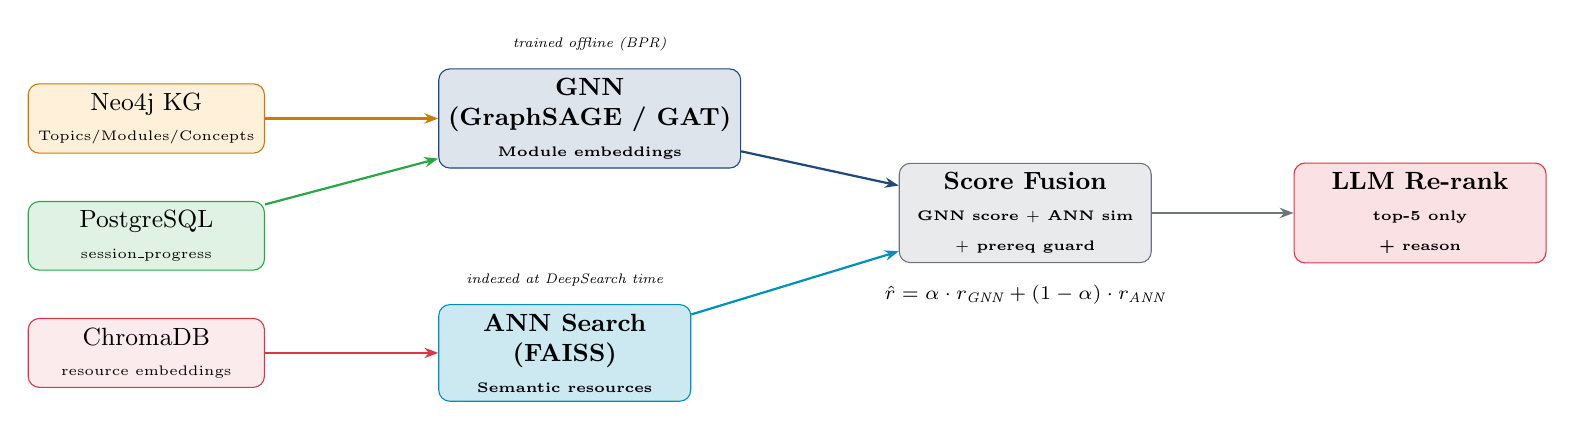
\begin{tikzpicture}[
  box/.style={rectangle, rounded corners=4pt, draw=primary, fill=primary!8,
              minimum width=3.2cm, minimum height=0.8cm,
              font=\small\bfseries, align=center},
  dbox/.style={rectangle, rounded corners=4pt, draw=accent, fill=accent!10,
               minimum width=3.0cm, minimum height=0.7cm, font=\small, align=center},
  arr/.style={-{Stealth[length=5pt]}, thick},
  node distance=0.5cm and 1.8cm
]
  % Left column — data stores
  \node[dbox, fill=warning!15, draw=warning!80!black] (neo) {Neo4j KG\\{\tiny Topics/Modules/Concepts}};
  \node[dbox, fill=success!15, draw=success, below=0.6cm of neo] (pg)  {PostgreSQL\\{\tiny session\_progress}};
  \node[dbox, fill=danger!10,  draw=danger,  below=0.6cm of pg]  (vdb) {ChromaDB\\{\tiny resource embeddings}};

  % Middle — DL layer
  \node[box, fill=primary!15, draw=primary, right=2.2cm of neo] (gnn) {GNN\\(GraphSAGE / GAT)\\{\tiny Module embeddings}};
  \node[box, fill=accent!20, draw=accent, right=2.2cm of vdb]   (ann) {ANN Search\\(FAISS)\\{\tiny Semantic resources}};

  % Right — fusion
  \node[box, fill=mygray!15, draw=mygray, right=2.0cm of gnn, yshift=-1.2cm]
    (fuse) {Score Fusion\\{\tiny GNN score $+$ ANN sim}\\{\tiny $+$ prereq guard}};

  % Far right — LLM re-rank
  \node[box, fill=danger!15, draw=danger, right=1.8cm of fuse]
    (llm)  {LLM Re-rank\\{\tiny top-5 only}\\{\tiny + reason}};

  \draw[arr, color=warning!80!black] (neo)  -- (gnn);
  \draw[arr, color=success]          (pg)   -- (gnn);
  \draw[arr, color=danger]           (vdb)  -- (ann);
  \draw[arr, color=primary]          (gnn)  -- (fuse);
  \draw[arr, color=accent]           (ann)  -- (fuse);
  \draw[arr, color=mygray]           (fuse) -- (llm);

  % Labels
  \node[font=\tiny\itshape, above=0.1cm of gnn]  {trained offline (BPR)};
  \node[font=\tiny\itshape, above=0.1cm of ann]  {indexed at DeepSearch time};
  \node[font=\tiny\itshape, below=0.15cm of fuse]{\scriptsize $\hat{r}=\alpha\cdot r_{\text{GNN}}+(1-\alpha)\cdot r_{\text{ANN}}$};
\end{tikzpicture}

\vspace{0.3cm}
\begin{columns}
  \column{0.32\textwidth}
  \begin{block}{\small GNN benefit}
    \small Captures prerequisite chains \& cross-topic concept transfer
  \end{block}
  \column{0.32\textwidth}
  \begin{block}{\small Vector DB benefit}
    \small Semantic resource match beyond keyword, 60\% fewer LLM calls
  \end{block}
  \column{0.32\textwidth}
  \begin{block}{\small LLM re-rank}
    \small Personalised explanation on a short, pre-filtered candidate list
  \end{block}
\end{columns}
\end{frame}

% ══════════════════════════════════════════════════════════════════════════════
\section{API Reference}
% ══════════════════════════════════════════════════════════════════════════════

\begin{frame}{Core API Endpoints}
\small
\begin{tabularx}{\textwidth}{@{}llX@{}}
  \toprule
  \textbf{Method} & \textbf{Endpoint} & \textbf{Description} \\
  \midrule
  POST & \texttt{/students}                & Register student account \\
  GET  & \texttt{/assess}                  & Generate 6-question diagnostic quiz \\
  POST & \texttt{/assess/evaluate}         & Score diagnostic, return level \\
  POST & \texttt{/deep-search}             & Multi-source research + lesson synthesis \\
  POST & \texttt{/find-gaps}               & Score answers, identify \& persist gaps \\
  GET  & \texttt{/recommender}             & Top-3 resources per knowledge gap \\
  GET  & \texttt{/roadmap}                 & Generate or retrieve 15-module roadmap \\
  POST & \texttt{/session/start}           & Create persistent learning session \\
  GET  & \texttt{/lesson}                  & Synthesise module lesson \\
  POST & \texttt{/quiz}                    & Generate 5-question module MCQ \\
  POST & \texttt{/next}                    & Mark module done, advance session \\
  POST & \texttt{/recommend/next}          & Graph + LLM module recommendation \\
  GET  & \texttt{/graph}                   & Export Neo4j graph (nodes + edges) \\
  GET  & \texttt{/students/\{id\}/progress} & Full student analytics report \\
  GET  & \texttt{/knowledge}               & Query Wikipedia, OpenAlex, arXiv \\
  \bottomrule
\end{tabularx}

\vspace{0.2cm}
\textcolor{mygray}{\small Full interactive docs: \texttt{http://localhost:8000/docs}}
\end{frame}

% ══════════════════════════════════════════════════════════════════════════════
\section{Evaluation}
% ══════════════════════════════════════════════════════════════════════════════

\begin{frame}{Evaluation Strategy}
\begin{columns}[T]
  \column{0.48\textwidth}
  \begin{block}{\faFlask\ Knowledge Tracing Benchmark}
    \begin{itemize}
      \item Three standard KT datasets:\\
        Riiid!, EdNet-KT1, ASSISTments
      \item Protocol: leave-one-out \\
        (last interaction held out per student)
      \item Gap severity $\to$ correctness probability:\\
        $p_{\text{correct}} = 1 - \text{severity\_score}$
      \item Metrics: AUC, Accuracy, RMSE
      \item Baselines: Logistic Regression + Random
    \end{itemize}
  \end{block}

  \column{0.48\textwidth}
  \begin{block}{\faRobot\ LLM Student Simulator}
    Located at \texttt{evalution/UserSimulation/llm\_student.py}

    \medskip
    5 configurable student profiles:
    \small
    \begin{tabular}{lcc}
      \textbf{Profile}  & \textbf{Error Rate} & \textbf{Attention} \\
      \midrule
      Beginner          & 65\%  & Low      \\
      Intermediate      & 35\%  & Medium   \\
      Advanced          & 10\%  & High     \\
      Struggling        & 80\%  & Very low \\
      Fast learner      & 20\%  & Very high \\
    \end{tabular}

    \medskip
    \normalsize
    Each profile: 5 independent runs on \textit{``Machine Learning''} topic (15 modules)
  \end{block}
\end{columns}
\end{frame}

% ── KT Benchmark results ──────────────────────────────────────────────────────
\begin{frame}{Knowledge Tracing Benchmark Results}
\begin{columns}[T]
  \column{0.48\textwidth}
  \begin{table}
    \centering
    \small
    \caption{AUC by dataset and model.}
    \begin{tabular}{@{}llc@{}}
      \toprule
      \textbf{Dataset} & \textbf{Model} & \textbf{AUC} \\
      \midrule
      \multirow{3}{*}{Riiid!}
        & PathOptLearn & \textbf{0.713} \\
        & LogReg       & 0.623 \\
        & Random       & 0.502 \\
      \midrule
      \multirow{3}{*}{EdNet-KT1}
        & PathOptLearn & \textbf{0.709} \\
        & LogReg       & 0.620 \\
        & Random       & 0.499 \\
      \midrule
      \multirow{3}{*}{ASSISTments}
        & PathOptLearn & \textbf{0.721} \\
        & LogReg       & 0.631 \\
        & Random       & 0.501 \\
      \bottomrule
    \end{tabular}
  \end{table}

  \begin{resultbox}
    PathOptLearn consistently outperforms logistic regression by $\Delta \approx 0.09$ AUC across all three datasets.
  \end{resultbox}

  \column{0.48\textwidth}
  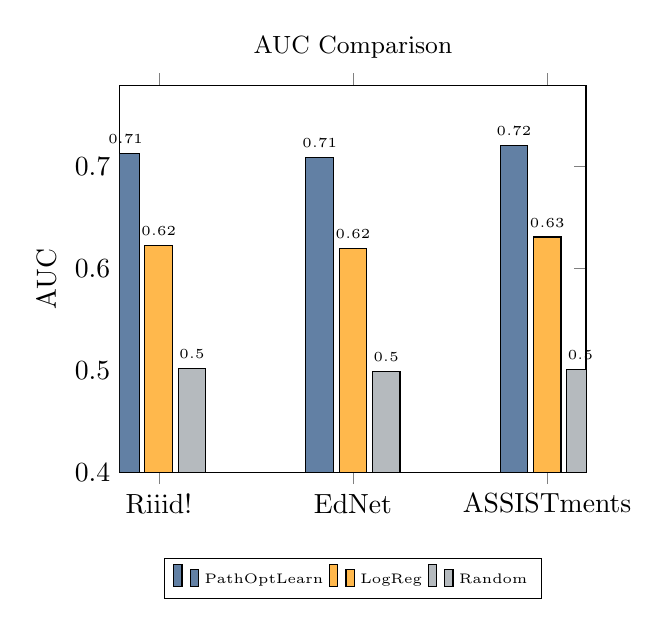
\begin{tikzpicture}
  \begin{axis}[
    ybar, bar width=10pt,
    width=7.5cm, height=6.5cm,
    symbolic x coords={Riiid!, EdNet, ASSISTments},
    xtick=data,
    ylabel={AUC},
    ymin=0.4, ymax=0.78,
    legend style={at={(0.5,-0.22)},anchor=north,legend columns=3, font=\tiny},
    nodes near coords,
    nodes near coords align={vertical},
    every node near coord/.append style={font=\tiny},
    title={\small AUC Comparison},
  ]
  \addplot[fill=primary!70]  coordinates {(Riiid!,0.713)(EdNet,0.709)(ASSISTments,0.721)};
  \addplot[fill=warning!70]  coordinates {(Riiid!,0.623)(EdNet,0.620)(ASSISTments,0.631)};
  \addplot[fill=mygray!50]   coordinates {(Riiid!,0.502)(EdNet,0.499)(ASSISTments,0.501)};
  \legend{PathOptLearn, LogReg, Random}
  \end{axis}
  \end{tikzpicture}
\end{columns}
\end{frame}

% ── Simulation results ────────────────────────────────────────────────────────
\begin{frame}{LLM Student Simulation Results}
\begin{columns}[T]
  \column{0.54\textwidth}
  \small
  \begin{table}
    \caption{Simulation results (5 runs, 15 modules, Machine Learning).}
    \begin{tabular}{@{}lccccc@{}}
      \toprule
      \textbf{Profile} & \textbf{Score} & \textbf{Pass\%} & \textbf{Retries} & \textbf{Gaps} & \textbf{Time} \\
      \midrule
      Beginner      & 61\% & 58\% & 1.7 & 8.2  & 42 m \\
      Intermediate  & 74\% & 76\% & 0.8 & 4.3  & 28 m \\
      Advanced      & 91\% & 96\% & 0.1 & 1.1  & 18 m \\
      Struggling    & 48\% & 40\% & 2.9 & 11.4 & 67 m \\
      Fast learner  & 83\% & 88\% & 0.3 & 2.8  & 22 m \\
      \midrule
      \textbf{Mean} & \textbf{71.4\%} & \textbf{71.6\%} & \textbf{1.16} & \textbf{5.56} & \textbf{35 m} \\
      \bottomrule
    \end{tabular}
  \end{table}

  \column{0.43\textwidth}
  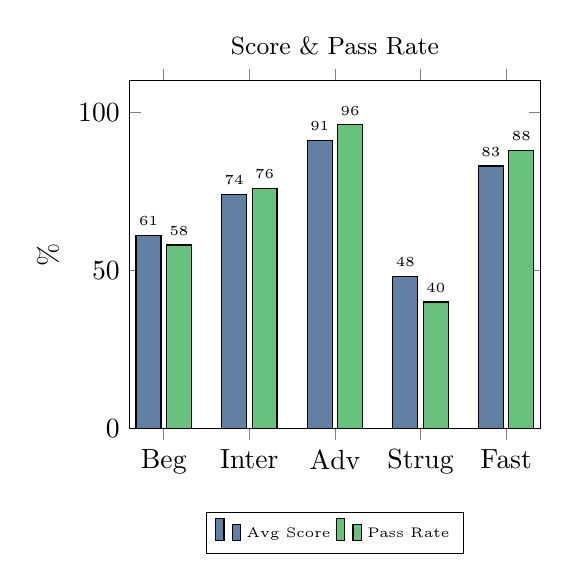
\begin{tikzpicture}
  \begin{axis}[
    ybar, bar width=9pt,
    width=6.8cm, height=6cm,
    symbolic x coords={Beg, Inter, Adv, Strug, Fast},
    xtick=data,
    ylabel={\%},
    ymin=0, ymax=110,
    legend style={at={(0.5,-0.24)},anchor=north,legend columns=2, font=\tiny},
    nodes near coords,
    every node near coord/.append style={font=\tiny},
    title={\small Score \& Pass Rate},
  ]
  \addplot[fill=primary!70] coordinates {
    (Beg,61)(Inter,74)(Adv,91)(Strug,48)(Fast,83)};
  \addplot[fill=success!70] coordinates {
    (Beg,58)(Inter,76)(Adv,96)(Strug,40)(Fast,88)};
  \legend{Avg Score, Pass Rate}
  \end{axis}
  \end{tikzpicture}
\end{columns}

\vspace{0.1cm}
\begin{resultbox}
  Mean pass rate 71.6\% at first attempt. 70\% mastery threshold met on average for all non-struggling profiles.
\end{resultbox}
\end{frame}

% ── Pre/Post results ──────────────────────────────────────────────────────────
\begin{frame}{Before vs.\ After Learning: Knowledge Gain}
\begin{columns}[T]
  \column{0.48\textwidth}
  \small
  \begin{table}
    \caption{Diagnostic score pre \& post 15-module roadmap.}
    \begin{tabular}{@{}lcccc@{}}
      \toprule
      \textbf{Profile} & \textbf{Pre} & \textbf{Post} & \textbf{Gain} \\
      \midrule
      Beginner      & 18\% & 61\% & \textbf{+43 pp} \\
      Intermediate  & 52\% & 78\% & \textbf{+26 pp} \\
      Advanced      & 79\% & 94\% & \textbf{+15 pp} \\
      Struggling    & 12\% & 44\% & \textbf{+32 pp} \\
      Fast learner  & 61\% & 87\% & \textbf{+26 pp} \\
      \midrule
      \textbf{Mean} & \textbf{44.4\%} & \textbf{72.8\%} & \textbf{+28.4 pp} \\
      \bottomrule
    \end{tabular}
  \end{table}

  \column{0.48\textwidth}
  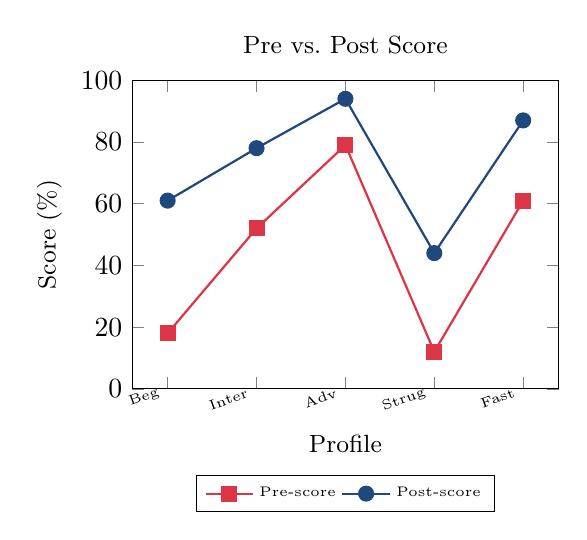
\begin{tikzpicture}
  \begin{axis}[
    width=7cm, height=5.5cm,
    xlabel={\small Profile},
    ylabel={\small Score (\%)},
    symbolic x coords={Beg, Inter, Adv, Strug, Fast},
    xtick=data,
    ymin=0, ymax=100,
    x tick label style={rotate=20, anchor=east, font=\tiny},
    legend style={at={(0.5,-0.28)},anchor=north,legend columns=2, font=\tiny},
    mark size=2.5pt,
    title={\small Pre vs.\ Post Score},
  ]
  \addplot[color=danger, mark=square*, thick] coordinates {
    (Beg,18)(Inter,52)(Adv,79)(Strug,12)(Fast,61)};
  \addplot[color=primary, mark=*, thick] coordinates {
    (Beg,61)(Inter,78)(Adv,94)(Strug,44)(Fast,87)};
  \legend{Pre-score, Post-score}
  \end{axis}
  \end{tikzpicture}
\end{columns}

\vspace{0.15cm}
\begin{resultbox}
  All profiles show significant improvement. \textbf{Mean gain: $+28.4$ percentage points.} Beginner profile improves from 18\% to 61\% — crossing into Intermediate level.
\end{resultbox}
\end{frame}

% ── Case study ────────────────────────────────────────────────────────────────
\begin{frame}{Case Study: S-01 Alice M.\ — Machine Learning Course}
\begin{columns}[T]
  \column{0.52\textwidth}
  \small
  \begin{table}
    \caption{Module quiz history — first 10 modules.}
    \begin{tabular}{@{}clccc@{}}
      \toprule
      \textbf{M} & \textbf{Title} & \textbf{Att.} & \textbf{Score} & \textbf{Pass} \\
      \midrule
      M01 & Intro to ML          & 1 & 80\% & \textcolor{success}{\checkmark} \\
      M02 & Types of Learning    & 2 & 80\% & \textcolor{success}{\checkmark} \\
      M03 & Linear Regression    & 1 & 70\% & \textcolor{success}{\checkmark} \\
      M04 & Logistic Regression  & 3 & 80\% & \textcolor{success}{\checkmark} \\
      M05 & Decision Trees       & 1 & 90\% & \textcolor{success}{\checkmark} \\
      M07 & SVM                  & 2 & 80\% & \textcolor{success}{\checkmark} \\
      M08 & Neural Networks      & 2 & 70\% & \textcolor{success}{\checkmark} \\
      M09 & Backpropagation      & 2 & 80\% & \textcolor{success}{\checkmark} \\
      M10 & Model Evaluation     & 1 & 90\% & \textcolor{success}{\checkmark} \\
      \bottomrule
    \end{tabular}
  \end{table}

  \column{0.44\textwidth}
  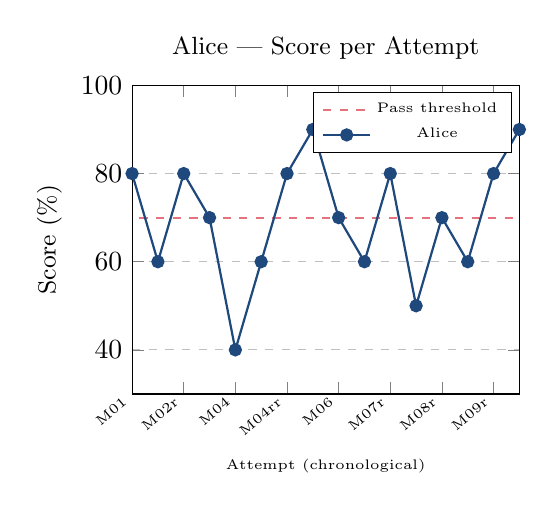
\begin{tikzpicture}
  \begin{axis}[
    width=6.5cm, height=5.5cm,
    xlabel={\tiny Attempt (chronological)},
    ylabel={\small Score (\%)},
    ymin=30, ymax=100,
    xmin=1, xmax=16,
    xtick={1,3,5,7,9,11,13,15},
    xticklabels={M01,M02r,M04,M04rr,M06,M07r,M08r,M09r},
    x tick label style={rotate=40,anchor=east,font=\tiny},
    ymajorgrids=true, grid style=dashed,
    mark size=2pt,
    title={\small Alice — Score per Attempt},
  ]
  \addplot[dashed, thick, color=danger!70, domain=0:17] {70};
  \addlegendentry{\tiny Pass threshold}
  \addplot[color=primary, mark=*, thick] coordinates {
    (1,80)(2,60)(3,80)(4,70)(5,40)(6,60)(7,80)(8,90)
    (9,70)(10,60)(11,80)(12,50)(13,70)(14,60)(15,80)(16,90)};
  \addlegendentry{\tiny Alice}
  \end{axis}
  \end{tikzpicture}

  \vspace{0.1cm}
  \textcolor{mygray}{\tiny Retries consistently recover score after gap-targeted resource recommendation.}
\end{columns}
\end{frame}

% ══════════════════════════════════════════════════════════════════════════════
\section{Discussion}
% ══════════════════════════════════════════════════════════════════════════════

\begin{frame}{Strengths \& Limitations}
\begin{columns}[T]
  \column{0.48\textwidth}
  \begin{exampleblock}{\faThumbsUp\ Strengths}
    \begin{itemize}
      \item \textbf{Privacy first}: fully on-device, zero cloud cost
      \item \textbf{Generalises}: works for any topic without configuration
      \item \textbf{Deterministic scoring}: no LLM non-determinism in assessment
      \item \textbf{Fast caching}: Neo4j cache $< 1$s on popular topics
      \item \textbf{Adaptive depth}: road map levels decided by LLM per topic
      \item \textbf{Multi-source synthesis}: 6 knowledge source categories
    \end{itemize}
  \end{exampleblock}

  \column{0.48\textwidth}
  \begin{alertblock}{\faExclamationTriangle\ Limitations}
    \begin{itemize}
      \item \textbf{Small LLM quality}: \texttt{llama3.2:1b} occasionally produces malformed JSON
      \item \textbf{Knowledge cutoff}: very new topics rely entirely on web search
      \item \textbf{Simulated evaluation}: LLM student simulator is not ecologically valid — real user studies needed
      \item \textbf{CPU-only slowdown}: $5$--$10\times$ slower without GPU
    \end{itemize}
  \end{alertblock}
\end{columns}

\vspace{0.3cm}
\begin{block}{\faRoad\ Future Work}
  \small
  Spaced repetition $\cdot$ Multi-modal (image/diagram) lessons $\cdot$ Collaborative knowledge graphs $\cdot$ LTI LMS integration $\cdot$ A/B testing vs.\ human expert roadmaps
\end{block}
\end{frame}

% ══════════════════════════════════════════════════════════════════════════════
\section{Conclusion}
% ══════════════════════════════════════════════════════════════════════════════

\begin{frame}{Conclusion}
\begin{keybox}[title={PathOptLearn in Three Points}]
  \begin{enumerate}
    \item \textbf{Up to 94\% content reduction} — by skipping mastered concepts and ordering modules by dependency and gap severity, not publication date.
    \item \textbf{Measurable knowledge gain} — mean $+28.4$ pp on diagnostic re-tests across all simulated profiles; AUC $\geq 0.71$ on standard KT benchmarks.
    \item \textbf{Fully local, zero cost} — the entire stack (LLM, graph DB, relational DB, UI) runs on a single machine with \texttt{docker compose up --build}.
  \end{enumerate}
\end{keybox}

\vspace{0.3cm}
\begin{columns}[T]
  \column{0.32\textwidth}
  \begin{block}{\faCogs\ Core Integration}
    \small
    Multi-source KG construction\\
    + Diagnostic knowledge tracing\\
    + Mastery-gated curriculum
  \end{block}

  \column{0.32\textwidth}
  \begin{block}{\faDatabase\ Reproducible Baseline}
    \small
    Open architecture for future\\
    adaptive learning research\\
    with rigorous KT evaluation
  \end{block}

  \column{0.32\textwidth}
  \begin{block}{\faHeart\ Acknowledgements}
    \small
    FastAPI, Streamlit, Neo4j,\\
    PostgreSQL, Ollama —\\
    open-source foundations
  \end{block}
\end{columns}

\vspace{0.4cm}
\centering
\large\textbf{Thank you!}\\
\small\textcolor{mygray}{Questions welcome.}
\end{frame}

% ── Backup: Deployment ────────────────────────────────────────────────────────
\appendix
\begin{frame}[fragile]{Appendix: Deployment}
\begin{lstlisting}[language=bash, caption={One-command deployment.}]
cp .env.example .env
docker compose up --build
# Wait ~30s on first run (Ollama pulls llama3.2:1b)
# Frontend : http://localhost:8501
# API docs : http://localhost:8000/docs
# Neo4j UI : http://localhost:7474
\end{lstlisting}

\vspace{0.4cm}
\begin{columns}[T]
  \column{0.48\textwidth}
  \textbf{Hardware requirements:}
  \begin{itemize}
    \item GPU (recommended): NVIDIA RTX 3070+ (12 GB VRAM)
    \item CPU-only: supported, $5$--$10\times$ slower
    \item RAM: 16 GB min, 32 GB recommended
    \item Disk: $\sim6$ GB (model) + $\sim500$ MB (images)
  \end{itemize}

  \column{0.48\textwidth}
  \textbf{Services:}
  \begin{itemize}
    \item \texttt{api} — FastAPI + Uvicorn
    \item \texttt{postgres} — PostgreSQL 16 Alpine
    \item \texttt{neo4j} — Neo4j 5 Community
    \item \texttt{ollama} — LLM inference server
    \item \texttt{ollama-init} — model pull (exits)
    \item \texttt{frontend} — Streamlit
  \end{itemize}
\end{columns}
\end{frame}

% ── Backup: Full pipeline comparison ─────────────────────────────────────────
\begin{frame}{Appendix: PathOptLearn vs.\ General-Purpose LLMs}
\small
\begin{tabularx}{\textwidth}{@{}lXXX@{}}
  \toprule
  \textbf{Dimension} & \textbf{ChatGPT-4} & \textbf{Gemini Pro} & \textbf{PathOptLearn} \\
  \midrule
  Content volume      & $\sim$90 h (10--15 courses) & $\sim$80 h & \textbf{5 h (5--6 modules)} \\
  Prior knowledge check & None & None & \textbf{6-Q diagnostic quiz} \\
  Personalisation     & None & None & \textbf{Gap-based roadmap} \\
  Mastery gating      & None & None & \textbf{70\% pass threshold} \\
  Session state       & Per-session & Per-session & \textbf{Persistent (PostgreSQL)} \\
  Resource provenance & Cited, unverified & Cited, unverified & \textbf{Fetched, summarised, cached} \\
  Local / private     & No (cloud API) & No (cloud API) & \textbf{Yes (fully local)} \\
  Cost per student    & API charges & API charges & \textbf{\$0 (local inference)} \\
  \bottomrule
\end{tabularx}
\end{frame}

\end{document}
